% Schriftliche Ausarbeitung -- AP5 (Projektseminar, Computational Engineering M.Sc.)
% Gliederung gemaess Projektanweisung_Invertiertes_Pendel.md Abschnitt 3 (AP5).
% Formatierung gemaess Layout.pdf (Fachbereich IuM, Dr. Rzehak).

\documentclass[12pt,oneside,parskip=half]{scrbook}

% --- Sprache & Anfuehrungszeichen ---
\usepackage[ngerman]{babel}
\usepackage[autostyle=true,german=quotes]{csquotes}

% --- Seitenlayout: Raender 2,5/2,5/2 cm, 1,5-zeilig (Layout.pdf) ---
\usepackage[top=2.5cm,left=2.5cm,right=2.5cm,bottom=2cm]{geometry}
\usepackage{setspace}
\onehalfspacing

% --- Schrift: Palatino als LaTeX-Pendant zu "Palatino Linotype" (Layout.pdf) ---
\usepackage[T1]{fontenc}
\usepackage{mathpazo}

% --- Mathematik: nummerierte, am "=" ausgerichtete Formeln (Layout.pdf, DIN 1338) ---
\usepackage{amsmath}
\usepackage{amssymb}
\usepackage{mathtools}
\usepackage{siunitx}

% --- Abbildungen & Tabellen ---
\usepackage{graphicx}
\usepackage{caption}
\usepackage{booktabs}
\graphicspath{{images/}}

% --- Code-Ausschnitte (Python / Modelica) ---
\usepackage{listings}
\lstset{
  basicstyle=\ttfamily\small,
  breaklines=true,
  frame=single,
  numbers=left,
  numberstyle=\tiny,
  captionpos=b,
}

% --- Literaturverzeichnis ---
\usepackage[backend=biber,style=numeric,sorting=nyt]{biblatex}
\addbibresource{references.bib}

% --- Lebende Kolumnentitel (Layout.pdf: "ggf. Hauptueberschriften als lebende Kolumnentitel") ---
\usepackage[headsepline,automark]{scrlayer-scrpage}
\clearscrheadfoot
\ihead{\headmark}
\ohead{\pagemark}
\pagestyle{scrheadings}

% --- Verlinkung (moeglichst spaet laden) ---
\usepackage[colorlinks=true,linkcolor=black,citecolor=black,urlcolor=blue]{hyperref}
\usepackage{cleveref}

\begin{document}

\begin{titlepage}
\begin{center}

{\large
Fachbereich Ingenieurwissenschaften und Mathematik\\[2pt]
Hochschule Bielefeld -- University of Applied Sciences and Arts\\[2pt]
Computational Engineering (M.Sc.)
}

\vspace{2cm}
{\Large Projektseminar -- Schriftliche Ausarbeitung}\\[1cm]

\rule{\linewidth}{0.4pt}\\[0.4cm]
{\huge\bfseries [Titel der Ausarbeitung]}\\[0.4cm]
\rule{\linewidth}{0.4pt}

\vspace{3cm}

\begin{tabular}{ll}
Vorgelegt von:      & [Vorname Nachname] \\
Matrikelnummer:     & [Matrikelnummer] \\
Studiengang:        & Computational Engineering (M.Sc.) \\
Betreuende Person:  & [Titel Vorname Nachname] \\
\end{tabular}

\vfill
[Ort], \today

\end{center}
\end{titlepage}


\frontmatter
\tableofcontents
\listoffigures
% \listoftables

\mainmatter
% !TEX root = ../main.tex
% Kapitel 1: Einleitung und Motivation
% Quelle/Ausgangspunkt: Projektanweisung_Invertiertes_Pendel.md (Abschnitte 1-2), eigene Motivation.
\chapter{Einleitung und Motivation}
\label{ch:einleitung}
\section{Problemstellung und Benchmark-Charakter}
Das mechatornische System des invertierten Pendels in diesem Projekt besteht aus einem translatorisch gelagerten
Wagen auf einer horizontalen Schiene und einem daran befestigten Pendelstab, auf diesem Stab wirkt keine direkte Stellgröße.
Dieses System bestizt in der Regelungstechnik und der nichtlinearen Dynamik eine besondere Benchmark-Charakter zur Validierung von Regelungsalgorithmen/ mathematische Kontrollstrategien (vgl. Stand der Technik des invertierten Pendels und dessen Integration in das Python-Software-Ökosystem
). Die Komplexität der Stabilisierung des invertierten Pendels auf dem Wagen resultiert aus drei physikalischen Eigenschaften:
\begin{itemize}
    \item Das System ist unterbestimmt, da die zwei Freiheitsgrade (Wagenposition s und Pendelwinkel $\phi$) nur durch eine Stellgröße $\tau$ die auf den Wagen wirkt beeinflusst werden können.
    \item Die Dynamik des Systems ist nichtlinear, da die Bewegungsgleichungen des invertierten Pendels nichtlinear sind.
    \item Die Zielposition (Pendel aufrecht, $\phi = \tau$) ist ein instabiler Gleichgewichtszustand, bei der kleinste Störungen zu einem Umkippen des Pendels führen können.
\end{itemize}
Einen ersten visuellen Eindruck der Simulationsumgebung ist in Abbildung \ref{fig:pendulum_simulation_interactive} dargestellt.
\begin{figure}[htbp]
    \centering
    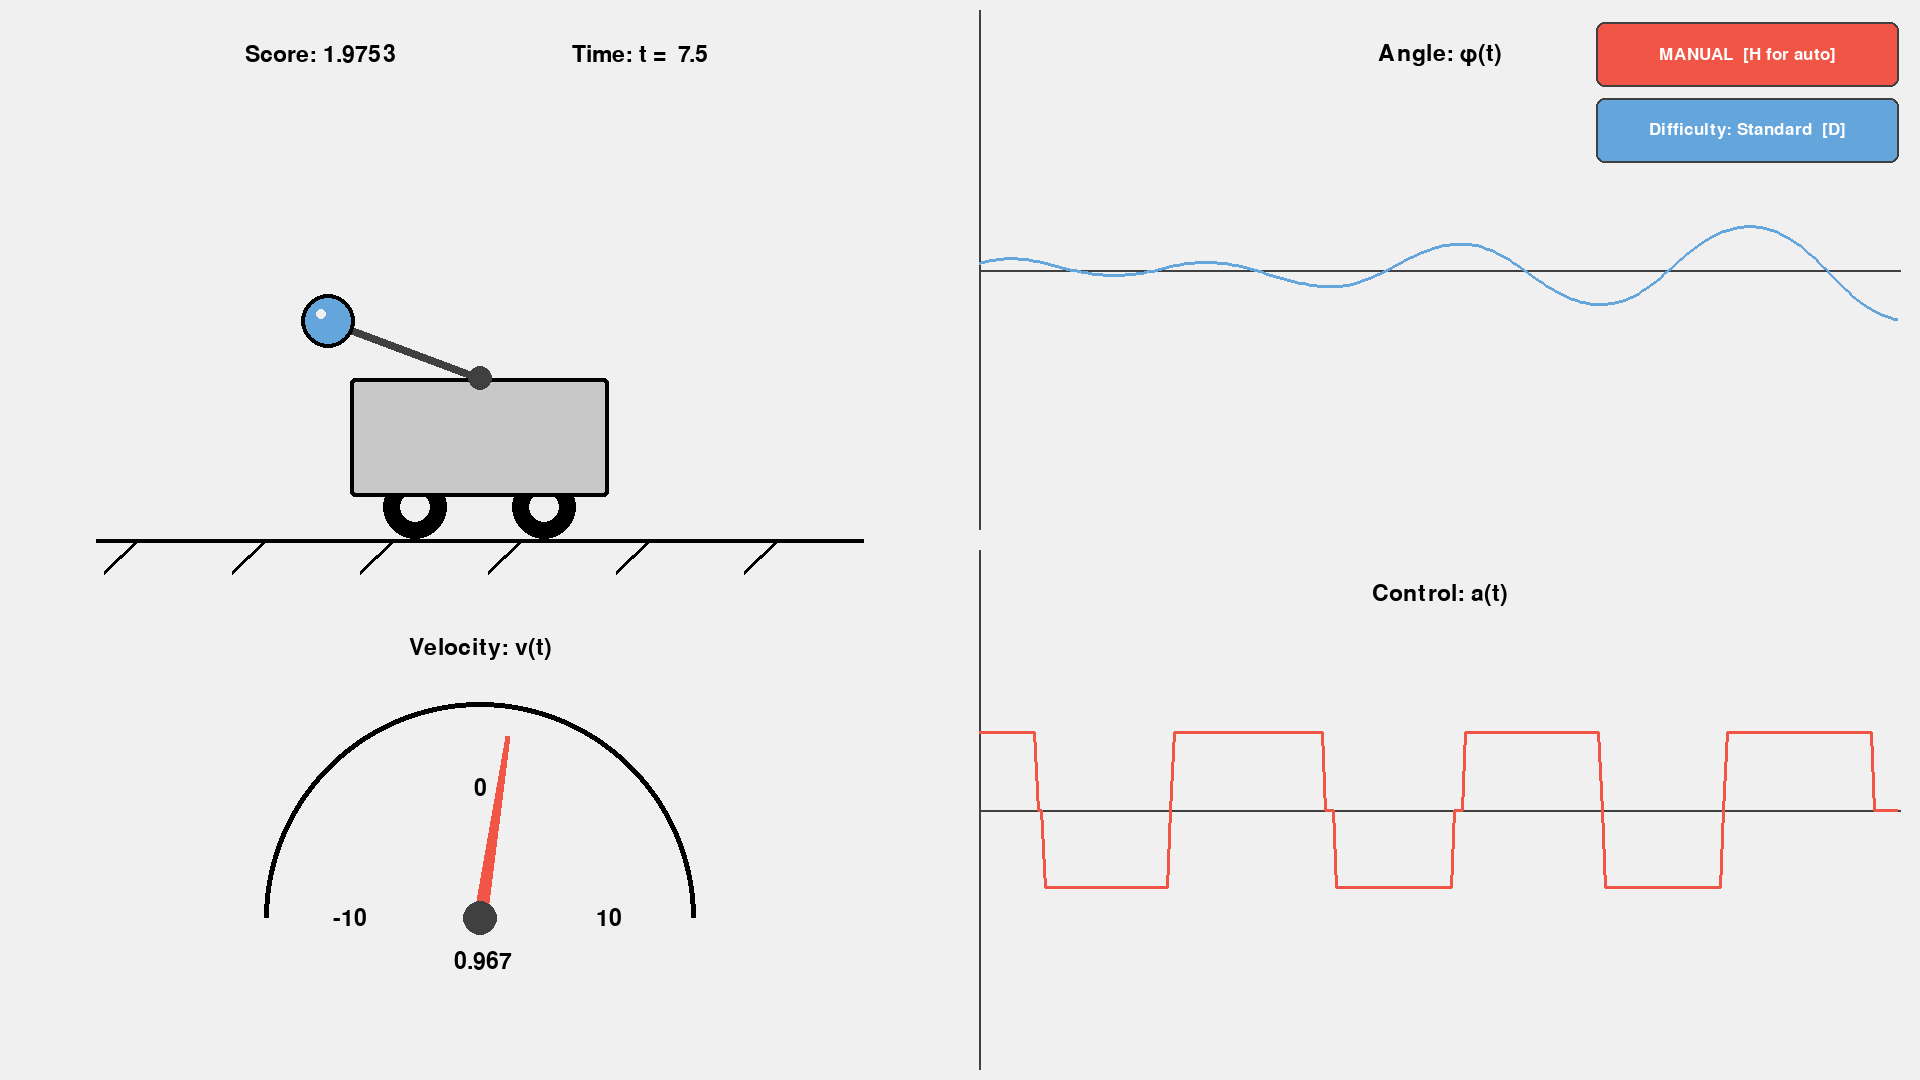
\includegraphics[width=0.75\textwidth]{game_interactive}
    \caption{Interaktive Simulationsumgebung des invertierten Pendels (Pygame-Fenster im laufenden Spiel).}
    \label{fig:pendulum_simulation_interactive}
\end{figure}

\section{Stand der Technik}
% mache ich später fertig

\section{Zielsetzung und Ausgangslage}
Das Ziel des Projekts ist die Weiterentwicklung eines unvollständigen, rein formalbasierten OpenModelica-Referenzmodells (pendulum.mo) zu einem physikalisch realistischen, interaktiven und spielbaren Simulationsumgebung. Darauf hin wurde auch die bestehnde Python-Simulationumgebung (pendulum\_game\_controlled.py) erweitert. 
Die Ausgangslage vor Bedinn des Projekts umfasste ein flaches Modelica-Modell des invertierten Pendels, das die Bewegungsgleichungen des Systems formal korrekt beschreibt, jedoch keine physikalisch realistische Simulation ermöglicht.
Im Rahmen dieses Projekts wurde das bestehende Referenzmodell durch eine objektorientierte Implementierung unter Verwendung der Modelica Standard Library (MSL), insbesondere der MultiBody-Bibliothek ersetzt um die gekoppelte Dynamik abzubilden.
Um die Interaktivität und Spielbarkeit zu gewährleisten, wurde die kompilierte Simulations-FMU in eine Python-Umgebung eingebunden.
Diese wurde um Tastensteuerung (Pause- und Reset-Funktion), ein zonebasiertes Punktesystem mit kontinuierlichkeits Bonus sowie Schwierigkeitsgrade erweitert.

\section{Aufbau der Arbeit}
Die Ausarbeitung dokumentiert den Entwicklungsprozess und ist in die folgenden Kapitel gegliedert:
\begin{itemize}
    \item Kapitel 2 widmet sich den theoretischen Grundlagen der Modellierung und der Herleitung der Bewegungsgleichungen über die Euler-Lagrange-Gleichungen her.
    \item Kapitel 3 beschreibt den Aufbau des MultiBody-Modells in OpenModelica sowie dessen algebraische Validierung.
    \item Kapitel 4 befasst sich mit der softwaretechnischen Umsetung der Simulationsumgebung der Spielmechaniken und des zonebasierten Punktesystems.
    \item Kapitel 5 stellt den Entwurf und die Implementierung der automatisierten PD-, LQR- und Swing-Up-Regler vor, zudem wird die Performance der Regler in verglichen.
    \item Kapitel 6 analysiert die physikalischen und spielerischen Auswirkungen der Schwierigkeitsgrade sowie die behebung des Resonanzproblems beim Scoring.
    \item Die Erkenntisse aus den vorherigen Kapiteln und Sovler-Eigenschaften werden in Kaptiel 7 diskuiert, bevor die Arbeit in Kapitel 8 mit einem Fazit und einem Ausblick schließt. 
\end{itemize}
    % TODO: Motivation, Zielsetzung des Projekts, Aufbau der Arbeit.

% !TEX root = ../main.tex
% Kapitel 2: Theoretische Grundlagen
% Quelle: protokoll.md (Lagrange-Herleitung, Linearisierung, Reglertheorie) -- NICHT erneut
% herleiten, hier einordnen/zusammenfassen und zitieren (siehe protokoll.md-Hinweis in
% Projektanweisung_Invertiertes_Pendel.md Zeile 17).
\chapter{Theoretische Grundlagen}
\label{ch:grundlagen}

\section{Mechanik des invertierten Pendels}
% TODO: Lagrange-Herleitung aus protokoll.md einordnen (Kurzfassung, Verweis statt Wiederholung).
% Winkelkonvention beachten: phi = 0 haengende, phi = pi aufrechte Lage (siehe CLAUDE.md).

\section{Regelungstechnik}
% TODO: Grundlagen zu PD-, LQR- und Swing-up-Regelung; Linearisierung um die aufrechte Lage
% (phi = pi), siehe protokoll.md.

% !TEX root = ../main.tex
% Kapitel 3: Modellierung mit Standardbibliotheken
% Quelle: AP1_Validierung.md
\chapter{Modellierung mit Standardbibliotheken}
\label{ch:modellierung}

\section{Vorgehen}
% TODO: MultiBody-Modell vs. formelbasiertes Modell, FMU-Export (Euler-Solver, siehe
% CLAUDE.md-Konvention "FMU solver").

\section{Herausforderungen}
% TODO: CVODE-Crash unter Windows/fmpy (AP1_Validierung.md Abschnitt 3.3).
%
% TODO (offen, Backlog): Solver-Vergleich CVODE vs. Euler unter WSL/Linux -- falls bis zur
% Abgabe abgeschlossen, gehoert das Kernergebnis hierher (Machbarkeit/Stabilitaet des Exports
% unter WSL). Siehe CLAUDE.md "Ideen / Backlog" -> "CVODE-Solver-Vergleich via WSL". Kurzer
% Querverweis auf Kapitel 5 (Reglerentwurf und Vergleich) fuer die Auswirkung auf die
% Reglerstabilitaet.

\section{Validierung}
% TODO: Validierungsmethodik (Momentanbeschleunigungsvergleich statt Trajektorienvergleich,
% AP1_Validierung.md Abschnitt 3.1-3.2).

% !TEX root = ../main.tex
% Kapitel 4: Umsetzung der Spielmechanik und des Punktesystems
% Quelle: AP2_Validierung.md, pendulum_game_controlled.py
\chapter{Umsetzung der Spielmechanik und des Punktesystems}
\label{ch:spielmechanik}

% TODO: Steuerung (Pfeiltasten / tau = +-MAX_TAU), Punktesystem (Toleranzzonen,
% Stability-Bonus), Auto/Manual/Mixed-Modus-Erkennung, Leaderboard (leaderboard.csv).

% !TEX root = ../main.tex
% Kapitel 5: Reglerentwurf und Vergleich
% Quelle: protokoll.md (Linearisierung), AP3_Reglervergleich.md
\chapter{Reglerentwurf und Vergleich}
\label{ch:reglerentwurf}

\section{PD-Regler}
% TODO: SimpleController; siehe AP3_Reglervergleich.md fuer die nachgewiesene Instabilitaet
% des geschlossenen Regelkreises nahe der aufrechten Lage (Eigenwertanalyse).

\section{LQR-Regler}
% TODO: Linearisierung um phi = pi (protokoll.md), Gain-Berechnung via
% scipy.linalg.solve_continuous_are.

\section{Swing-up-Regler}
% TODO: Energiepump-Regelgesetz und Hysterese-Umschaltung zum LQR (CAPTURE_THETA/RELEASE_THETA).

\section{Vergleich}
% TODO: Stabilitaet, Reaktionszeit und Robustheit aus AP3_Reglervergleich.md zusammenfassen.
%
% TODO (offen, Backlog): falls der Solver-Vergleich (Kapitel 3, Abschnitt "Herausforderungen")
% abgeschlossen ist, hier kurz einordnen, ob/wie sich die Reglerstabilitaet unter CVODE
% gegenueber Euler aendert.

% !TEX root = ../main.tex
% Kapitel 6: Schwierigkeitsgrade und deren Auswirkung
% Quelle: docs/superpowers/specs/2026-08-19-ap4-difficulty-levels-design.md,
% CLAUDE.md (AP4-Eintrag in "AP History")
\chapter{Schwierigkeitsgrade und deren Auswirkung}
\label{ch:schwierigkeitsgrade}

% TODO: Variationsachsen (Toleranzbereich, Masse/Reibung m_cart/m_pend/d_cart/d_pend),
% Auto/Manual-Isolation (H/D-Tasten), Playtest-Ergebnis (urspruengliche Leicht-Werte waren
% zu hart -- Score 0.0 -- und wurden nach interaktivem Test korrigiert, siehe CLAUDE.md
% AP-History 2026-08-19).

% !TEX root = ../main.tex
% Kapitel 7: Ergebnisse und Diskussion
\chapter{Ergebnisse und Diskussion}
\label{ch:ergebnisse}

% TODO: Uebergreifende Synthese ueber AP1-AP4 (keine reine Wiederholung der Einzelkapitel).

% !TEX root = ../main.tex
% Kapitel 8: Fazit und Ausblick
\chapter{Fazit und Ausblick}
\label{ch:fazit}

% TODO: Zusammenfassung der Ergebnisse.
% Ausblick-Ideen siehe CLAUDE.md "Ideen / Backlog": Doppelpendel, SwingUp-Regler faengt nach
% Ueberschwingen nicht mehr, CVODE-WSL-Solver-Vergleich (falls bis Abgabe noch offen).


\backmatter
\printbibliography[title={Literaturverzeichnis}]

% Anhang (zaehlt laut Layout.pdf nicht zum 20-Seiten-Textumfang, bleibt unnummeriert):
% \input{chapters/anhang}

\end{document}
